
In this section, we will present two analytic examples due to Le that are equivalent and belong to the class of spaces
called the first kind arithmetic expression space $\mathfrak{K}_1$.

\subsection{Example space I}\label{subsec:exmp1}

Consider the upper half plane ${\mathcal{H}: (x, y) \ | \ y > 0}$ equipped with an inner product and metrics defined as follows:

$$
\mathbf{a} \cdot \mathbf{b} = \begin{bmatrix} a_x & a_y \end{bmatrix} \begin{bmatrix} \frac{1}{y^2} & 0 \\ 0 & \frac{1}{y^2} \end{bmatrix} \begin{bmatrix} b_x \ b_y \end{bmatrix}
$$

and

$$
ds^2 = \frac{1}{y^2} (dx^2 + dy^2)
$$

We also consider an assignment function $A$ defined on $\mathcal{H}$ as follows\footnote{This analytic example is provided by Le Zhang, and the geometry interpretation is given by Mingli Yuan}:

\begin{equation}
A = - \frac{x}{y}
\end{equation}

\begin{theorem}\footnote{The proof is originally by Le Zhang, and modified by Mingli Yuan}
For the assignment $A$ defined by above formula, $A$ satisfy the flow equation\eqref{eq:flow}
\end{theorem}

\begin{proof}
$$
da = d(-\frac{x}{y}) = \frac{xdy - ydx}{y^2} = -\frac{dx + ady}{y}
$$

and

$$
ds = \frac{\sqrt{dx^2 + dy^2}}{y}
$$

then

$$
\frac{da}{ds} = - \frac{dx + ady}{y} \frac{y}{\sqrt{dx^2 + dy^2}} = - \frac{dx + ady}{\sqrt{dx^2 + dy^2}}
$$

Considering that the local coordinate is given by $(-1, 0)$ and $(0, -1)$ under the right-hand rule, we have:

$$
\cos \theta = \frac{\begin{bmatrix} dx & dy \end{bmatrix} \begin{bmatrix} \frac{1}{y^2} & 0 \\ 0 & \frac{1}{y^2} \end{bmatrix} \begin{bmatrix} -1 \\ 0 \end{bmatrix}}{\sqrt{\begin{bmatrix} dx & dy \end{bmatrix} \begin{bmatrix} \frac{1}{y^2} & 0 \\ 0 & \frac{1}{y^2} \end{bmatrix} \begin{bmatrix} dx \\ dy \end{bmatrix}}\sqrt{\begin{bmatrix} -1 & 0 \end{bmatrix} \begin{bmatrix} \frac{1}{y^2} & 0 \\ 0 & \frac{1}{y^2} \end{bmatrix} \begin{bmatrix} -1 \\ 0 \end{bmatrix}}}
$$

hence

$$
\cos \theta = \frac{-dx}{\sqrt{dx^2 + dy^2}}
$$

and similarly

$$
\sin \theta = \frac{-dy}{\sqrt{dx^2 + dy^2}}
$$

then

$$
\frac{da}{ds} = \cos \theta + a \sin \theta
$$

\end{proof}

We can verify $A$ is an eigenfunction of the Laplacian

$$
\Delta A = - y^2 (\frac{\partial^2}{\partial x^2} A + \frac{\partial^2}{\partial y^2} A) = y^2 (\frac{1}{\partial y} (\frac{1}{\partial y} \frac{x}{y})) = 2 A
$$

\subsection{A horocycle-based coordinate system}\label{subsec:horocyclebased}

First, we introduce the horocycle-based coordinate system for hyperbolic surfaces.
It is a global coordinate system given by two orthogonal sets of circles: one set consists of horocycles that share the same ideal point,
while the other consists of geodesics that are perpendicular to the first set.

On the Poincaré disc $\mathcal{P}$, the blue horocycles are tangible at the ideal point $\Omega$, forming the first set of circles.
The green lines are geodesics that form the second set. The coordinates of point $P$ are given by the lengths of $OQ$ and $QP$,
where point $O$ is the origin and the length is measured using the metric of the hyperbolic surface.

The coordinates of $P$ are $(u,v)$, where the sign of the length is determined by the following rules:
\begin{itemize}
\item u: if $P$ is on the same side of $\Omega$, then $u$ is positive; otherwise, $u$ is negative
\item v: the sign of the length should satisfy the right-hand rule
\end{itemize}

\begin{figure}[ht]
\centering
\resizebox{0.5\textwidth}{!}{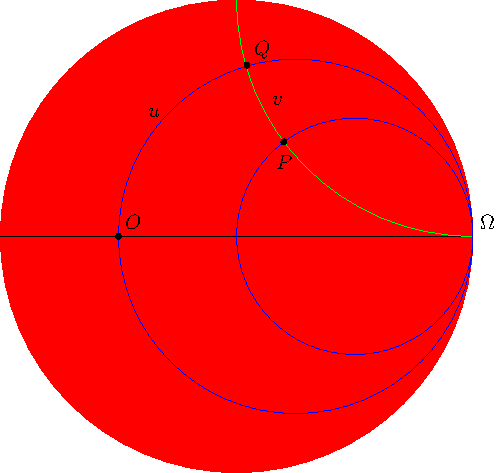
\includegraphics{images/11-horocyclebased}}
\caption{A horocycle-based coordinate system}\label{fig:horocyclecoord}
\end{figure}

We can equip it with an inner product

\[
\mathbf{a} \cdot \mathbf{b} = \begin{bmatrix} a_u & a_v \end{bmatrix} \begin{bmatrix} e^{-2v} & 0 \\ 0 & 1 \end{bmatrix} \begin{bmatrix} b_u \\ b_v \end{bmatrix}
\]

and the metrics

$$
ds^2 = e^{-2v} du^2 + dv^2
$$

Laplacian is given by\cite{Costa2001ADO}

$$
\Delta = e^{2v} \frac{\partial^2}{{\partial u}^2} + \frac{\partial^2}{{\partial v}^2} - \frac{\partial}{\partial v}
$$

\subsection{Example space II}\label{subsec:exmp2}

Giving the Poincaré disc $\mathcal{P}$ equipped with the above horocycle-based coordinate system,
we consider an assignment function $A$ defined on $\mathcal{P}$ as follows\footnote{This analytic example is provided by Le Zhang, and the geometry interpretation is given by Mingli Yuan}:

\begin{equation}
A = u e^{-v}
\end{equation}

\begin{theorem}
For the assignment $A$ defined by above formula, $A$ satisfy the flow equation\eqref{eq:flow}
\end{theorem}

\begin{figure}[ht]
\centering
\resizebox{0.8\textwidth}{!}{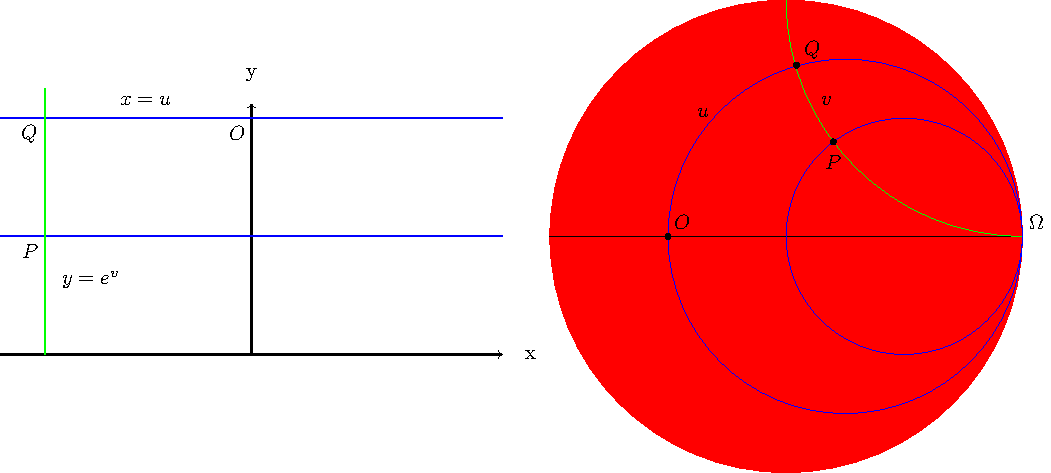
\includegraphics{images/12-proofbymapping}}
\caption{Mapping between two examples}\label{fig:mapping}
\end{figure}

\begin{proof}

If we introduce complex in the upper half plane model in last section \ref{subsec:exmp1}

$$
z = x + y i
$$

and stetup a Möbius transform between the upper half plane and current horocycle-based coordinate system:

$$
z \mapsto \frac{z-i}{z+i}
$$

This transform maps each horizontal lines in $\mathcal{H}$ into the horocycles sharing the same ideal point $\Omega = 1$ in $\mathcal{P}$,
also it maps each vertical geodesics in $\mathcal{H}$ into geodesics in $\mathcal{P}$ which are perpendicular to the above horocycles.

And rewrite the Möbius transform in the target coordinate, we get:

$$
\begin{cases}
x = u\\
y = e^v \\
\end{cases}
$$

This lead to

$$
A = -\frac{x}{y} = u e^{-v}
$$

And because of theorem \ref{thm:isometry} and Möbius transform is conformal, we can conclude that $A = u e^{-v}$ obey flow equation.

\end{proof}

We can verify $A$ is also an eigenfunction of the Laplacian
$$
\Delta A = e^{2v} \frac{\partial^2(u e^{-v})}{{\partial u}^2} + \frac{\partial^2(u e^{-v})}{{\partial v}^2} - \frac{\partial(u e^{-v})}{\partial v} = 2A
$$

From the above proof, we can see that the two assignment function $A$ arose from the same geometry setting, they are equivalent to each other.

\subsection{Generator independence}

Considering the upper half plane $\mathcal{B}$:
$$
\{\mathcal{B}: (x, y) | y > 0 \}
$$

equipped with an inner product and metrics as follows:

$$
\mathbf{a} \cdot \mathbf{b} = \begin{bmatrix} a_x & a_y \end{bmatrix} \begin{bmatrix} \frac{1}{\mu^2 y^2} & 0 \\ 0 & \frac{1}{\lambda^2 y^2} \end{bmatrix} \begin{bmatrix} b_x \\ b_y \end{bmatrix}
$$

$$
ds^2 = \frac{1}{y^2}(\frac{dx^2}{\mu^2} + \frac{dy^2}{\lambda^2})
$$

Whatever the choice of $\mu$ and $\lambda$, the assignment is given by

\begin{equation}
A = - \frac{x}{y}
\end{equation}

We can verify $A$ satisfying the flow equation\eqref{eq:flow}, and also it is generator independent.

\begin{theorem}
The above $A$ satisfying the flow equation\eqref{eq:flow}
\end{theorem}

\begin{proof}
$$
da = d(-\frac{x}{y}) = \frac{xdy - ydx}{y^2} = -\frac{dx + a dy}{y}
$$

Notice that

$$
ds = \frac{1}{y}\sqrt{\frac{dx^2}{\mu^2} + \frac{dy^2}{\lambda^2}}
$$

then

$$
\frac{da}{ds} = - \frac{dx + a dy}{y} \frac{y}{\sqrt{\frac{dx^2}{\mu^2} + \frac{dy^2}{\lambda^2}}} = \frac{dx + a dy}{\sqrt{\frac{dx^2}{\mu^2} + \frac{dy^2}{\lambda^2}}}
$$

Consider the local coordinate system given by $(-1, 0)$ and $(0, -1)$ according to the right-hand rule, we have

$$
\cos \theta = \frac{\begin{bmatrix} dx & dy \end{bmatrix} \begin{bmatrix} \frac{1}{\mu^2 y^2} & 0 \\ 0 & \frac{1}{\lambda^2 y^2} \end{bmatrix} \begin{bmatrix} -1 \\ 0 \end{bmatrix}}{\sqrt{\begin{bmatrix} dx & dy \end{bmatrix} \begin{bmatrix} \frac{1}{\mu^2 y^2} & 0 \\ 0 & \frac{1}{\lambda^2 y^2} \end{bmatrix} \begin{bmatrix} dx \\ dy \end{bmatrix}}\sqrt{\begin{bmatrix} -1 & 0 \end{bmatrix} \begin{bmatrix} \frac{1}{\mu^2 y^2} & 0 \\ 0 & \frac{1}{\lambda^2 y^2} \end{bmatrix} \begin{bmatrix} -1 \\ 0 \end{bmatrix}}}
$$

Therefore we have

$$
\cos \theta = \frac{-\frac{dx}{\mu}}{\sqrt{\frac{dx^2}{\mu^2} + \frac{dy^2}{\lambda^2}}}
$$

Similarly

$$
\sin \theta = \frac{-\frac{dy}{\lambda}}{\sqrt{\frac{dx^2}{\mu^2} + \frac{dy^2}{\lambda^2}}}
$$

Hence we have

$$
\frac{da}{ds} = \mu \cos \theta + a \lambda \sin \theta
$$

\end{proof}

\subsection{Related problems}

\emph{Eigenfunction problem}: TODO.

\emph{Eigenfunction and classification problem}: TODO.

\newpage
